%\documentclass[twocolumn]{article}
\documentclass{article}
\usepackage{CJKutf8}
\usepackage{amsmath}
\usepackage{graphicx}

\begin{document}
\begin{CJK}{UTF8}{gbsn}

\title{Advanced NLP Project 2 - Web People Search(WePS)}
\author{10848194 樊锴 \and 10848263 王晨}
%\author{10848194  \and 10848263 }
\date{May 16, 2009}

\maketitle

\section{Introduction}

    Please refer to official WePS website~\cite{weps} for more project introduction. \\
    There have been many early works~\cite{fleischman_multi-document_2004}~\cite{mann_unsupervised_2003} from which we have borrowed many thoughts.

\section{Methodology}

    To group web pages according to entities, our work compose of three major steps: 
    \begin{itemize}
    \item Feature Extraction, to extract features from original web pages. Here, 'feature' may refer to many different informations, like the main text, the named entities, or phone numbers within a page.
    \item Similarity Calculation, to find similarity between two web pages.
    \item Clustering, to form groups using the similarity of each page pair.
    \end{itemize}
    We describe each step in detail in following sections.

    \subsection{Feature Extraction}
        A feature is a kind of information to identify the web page. All the features we used are represented in the form of string vectors.
        Totally, we use 12 feature to describe a web page, and they can be devided into 3 categories.

        \subsubsection{Text Features}
            The basic idea of text features is that if two web pages are talking about the same person, then their content would be somewhat similar, anyway, we get most information from the web page through the text. However, there are different methods to choose the text, here we present 3 different ways. All these features are in the form of a text. When they are extracted, we tokenized these texts and represent them in term vectors.
            \begin{description}
            \item [Fulltext] The fulltext of a web page is composed of the all the text information we see in a web page, along with its title.
            \item [Summary] Many times, a web page will talk about things about many persons, so we hope to extact the content just related to the target person. So we devided the fulltext into sentences and retain sentences where the target person's name appears. An ideal way to do this would be using Pronoun Resolution to decide precisely what content is related, however, we failed to find a tool to accomplish this target, so we used the simple but less precise way. 
            \item [Metadata] Except texts, we think the matadata of a web page, including title, url, and description would also make sense, so we combined these information to form a metadata feature.
            \end{description}

        \subsubsection{Named Entity Features}
            We think Named Entities would be quite accurate to distinguish one person from another, for example, if two page indicate the same location and the same organization, then we are quite confident these two pages are indicating the same person. Here we don't consider the situation that different entities may share the same name. We extract three type of named entites(as provided by stanford NER tools):
            \begin{itemize}
            \item Person
            \item Organization
            \item Location
            \end{itemize}
            Each entity may contain more than one words. 
            It's not unusual that entities may have different forms, "University of Chicago" and "Chicago University" is just the same entity, "Jeorge Bush" and "Jeorge W. Bush" probably refer to the same people. 
            So we dicided to use each word instead of all words to represent an entity. \\
            Of course there is shortage for this method, for "Micheal Jackson" and "Micheal Jordan" is just different person, but they will share a same entity "Michael". Besides, while two "FBI"s will share a single entity, "Federal Bureau of Investigation" share four entities. 
            We have not precisely evaluated which method would perform better, and choose the single word way just because it is simpler.

        \subsubsection{Rugular Expression Features}
            We try to use regular expression to extract more information from text, hoping these features would help differentiate different "target person".
            \begin{description}
            \item [URL] 
            \begin{verbatim} 
            "(news|telnet|nttp|file|http|ftp|https)://([-A-Za-z0-9]+\.[-A-Za-z0-9\.]+)(:[0-9]*)?(/[-A-Za-z0-9_\$\.\+\!\*\(\),;:@&=\?/~\#\%]+)*/?"
            \end{verbatim} 
            It is easy to understand if two web pages share a lot of links and urls, they may have a strong relation in contents, and therefore quite probable to indicate to the same person.
            So we extract urls from the web pages, including urls in background links and urls contained in texts. 
            Also we include the page's own url. 
            After the urls is find, we remove all non-ascii characters and replace the '/' and '.' to space to form a plain text.
            \item [Email]
            \begin{verbatim} 
            "(mailto:)?([-A-Za-z0-9]+@([-A-Za-z0-9]+\.[-A-Za-z0-9\.]+))"
            \end{verbatim} 
            If two page share a same email address in texts or background links, they are prabably refer to one person. We use the same text base as for URL to extract email addresses. All following processes are also similar.
            \item [Domain]
            While URLs and Emails may be accurate, they are usually sparce. So we leveraged the domain of these URLs and Emails to form a less accurate but denser feature, and expect this feature to have better effect in reality.
            \item [Number]
            \begin{verbatim} 
            "(\d|-){2,}"
            \end{verbatim} 
            We want to extract number informations like birthday, age, room number or telephone number, but it's quite difficult to tell one from another, so we use a naive approach, extract all numbers from the text.
            \item [Telephone number]
            \begin{verbatim} 
            "\d(\d|-){5,}"
            \end{verbatim} 
            It's difficult to tell exactly what number is a telephone number, so se just use a rough regular expression.
            \item [Year]
            \begin{verbatim} 
            "[^0-9]1\d\d\d[^0-9]"
            \end{verbatim} 
            Again, we just use a naive approach, treat all 4-digit numbers start with '1' as a indication of year.
            \end{description}

    \subsection{Similarity Calculation}
        We want to calculate a similarty between each page pair. 
        At first we would calculate a similarity for each feature. \\
        For text features, Vector Space Model plus Cosine Similarty should is an easy choice.
        For named entity features and regular expression features, we first tried to treat each feature as a word set, and use size of intersection and "Jaccard Coefficient" to measure similarity. 
        However, consider the way we construct the above features, "pku" definitely carry more information than "com" in a domain feature, also is "prinston" to "university" in named entity features.
        While set intersection or "Jaccard Coefficient" don't address these differences, Vector Space Model do.
        So finally, we decide to use Vector Space Model for all features and calculate the Cosine Similarity as the similarity for each pair.
        \subsubsection{Vector Space Model}
            To realize Vector Space Model, we used a  stop word list to filter stop words, and stem all remaining words, then apply TF-IDF process.
            Since we write our program in Python and VSM calculation is very computation-intensive, we use the NumPy library to carry out main computation, which would speed up the calculation for one order of magnitude.

        \subsubsection{Learning Similarity}
            Although we have calculated the similarilty for each feature, we would like to integrate them to one single metric which could be used to represent the similarity between pages. 
            One possible way would be interpolation, however since there are many features it is difficult to determine parameters. \\
            We use machine learning method instead. 
            Since we have calculate similarity of each feature for each page pair, and with the training set we would have known whether such page pair is really related to one person. 
            So we could train a model, which take as input the similarity of each feature for a page pair and output the possibility that such pair should be labeled as one person. \\
            We tried different machine learning methods, like Maximum Entropy, Naive Bayes and Decision Trees.
            With each method, we finally got a similarity for each page pair. 

    \subsection{Clustering}
        Now that we have got a similarity for each pair, we still need to find a way to cluster pages so that all pages within one group is related to the same person and pages from different groups should be related to different person.
        One method is K-Means clustering, and we only need to decide how many clusters should there be. 
        However, it is just difficult to find a best cluster number.
        Another method is Hierarchical Agglomerative Clustering, with which we need to decide the similarity threshold used to stop clustering.
        We implemented both algorithms, and tried to find a best parameter.

    \subsection{Other Issues}
        While processing documents, we find the recognization of discard pages a difficult problem. 
        In our program, we just discard any pages whose summary is short than 5 words.
        When we check the results, we find this is not sufficient, and when there are many discarded pages, the result is poor.
        We haven't figure out a better way, but we tried to use the discarded items in the truth files as a priori, and compared the results.

\section{Environment and Tools}

    Our project is totally completed in Linux environment, and is mainly written in Python, however, some shell scripts is also written to use thirdparty tools.

    Here is a list of programs and tools needed to run our project:
    \begin{itemize}
    \item Utuntu 8.04 and Python 2.5 is our major programming platform.
    \item NumPy\footnote{http://numpy.scipy.org}, a python package for scientific calculation, used in Vector Space Model calculation.
    \item Psyco\footnote{http://psyco.sourceforge.net}, a python extension used to speed up python execution.
    \item Jericho HTML Parser\footnote{http://jerichohtml.sourceforge.net}, used to extract text and url links from original web pages.
    \item Stanford Named Entity Recognizer\footnote{http://nlp.stanford.edu/ner/}, used to extract named entities from texts.
    \item Natural Languate Toolkit(NLTK)\footnote{http://www.nltk.org} is a python software providing a lot of NLP algorithms and datasets. We used just a tiny part of its utilities, including Sentence Tokenizing, Word Tokenizing, english stop word list, and Porter Stemmer.
    \end{itemize}

    Our own program files includes:
    \begin{description}
    \item [prep.sh] This is a  Bash Shell script used to prepare the text and entities, through calling Jericho HTML Parser and Stanford NER tools.
    \item [nlp.py] This is a python script used a library, including a series of utilies used to fullfill this project, like VSM calculation, K-Means clustering, HAC clusting, regular expression extraction, and so on.
    \item [weps.py] This python script including the mainflow of our project. Its functions are splitted to three part: feature extraction and similarity calculation through VSM, similarity learing, and clustering.
    \item [score.sh] A trivial utility to collect final scores.
    \end{description}

    To run our program, one should run \em{./prep.sh} first, then run \em{./weps.py -pmc} to carry out the main process, and finally run \em{./score.sh} to collect scores.
    All intermediate results is storeded in \em{./tmp} directory.
    Typically, it takes hours for our programs to run completely.

\section{Experiments and Results}
    We try out all features, with different learning methods, different clustering methods and different parameters. \\
    \begin{figure}
    \caption{F-0.5 Measure change with cluster number in K-Means clustering}
    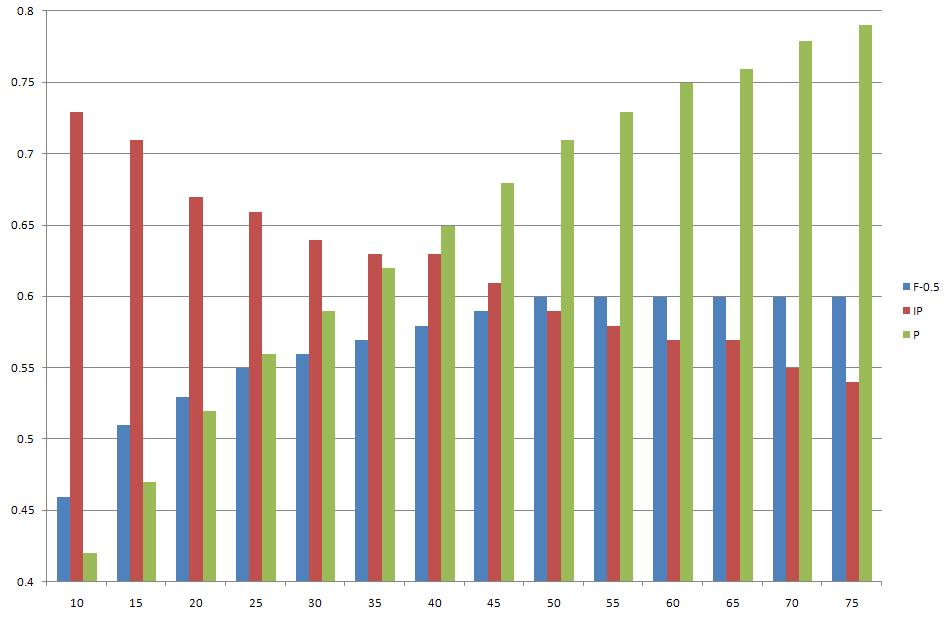
\includegraphics[width=120mm]{kmeans}
    \label{fig:kmeans}
    \end{figure}

    \begin{figure}
    \caption{F-0.5 Measure change with threshold in HAC clustering}
    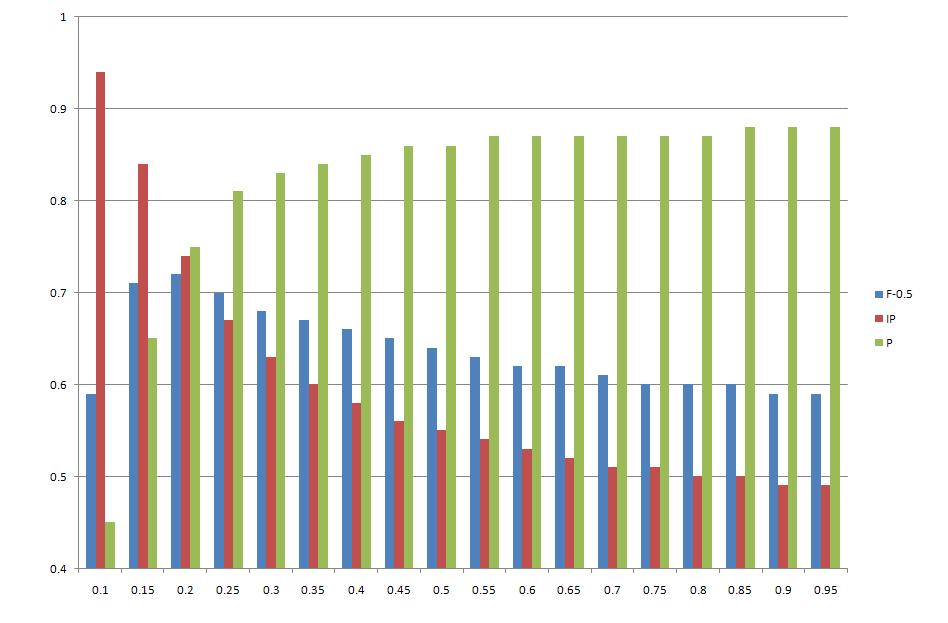
\includegraphics[width=120mm]{agglo}
    \label{fig:agglo}
    \end{figure}

    Figure~\ref{fig:kmeans} and Figure~\ref{fig:agglo} show the F-0.5 Measure change with parameters for a single feature in different clustering methods.
    We found that HAC generally performed better than K-Means, thus our following results are all based on HAC clustering. \\
    
    \begin{figure}
    \caption{Best F-0.5 Measure for different similarity type}
    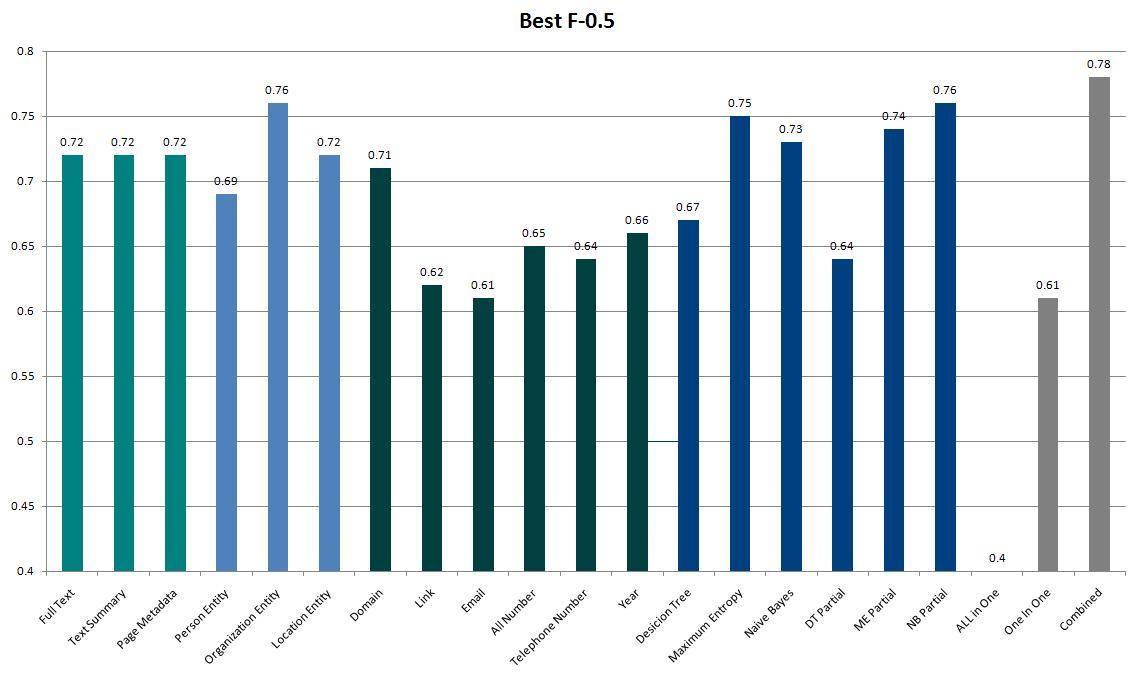
\includegraphics[width=120mm]{best}
    \label{fig:best}
    \end{figure}

    \begin{figure}
    \caption{Comparison of whether take discared items as priori}
    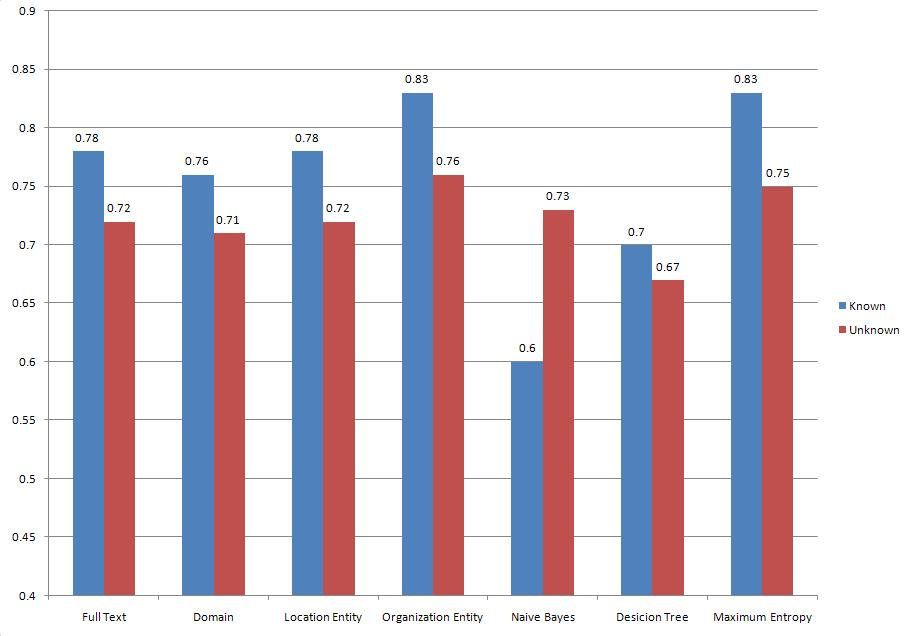
\includegraphics[width=120mm]{discard}
    \label{fig:discard}
    \end{figure}

    Figure~\ref{fig:best} showed the best result we got for different features.  
    Generally speaking, named entity features had the best performance, while text features also performed well. 
    In contract, regular expression features had the worst performance, we think it's partly because the extraction is not precise enough, and partly because the features is too sparce. \\

    Figure~\ref{fig:discard} show the comparson of results whether we take discarded items as a priori. It's clear that the discarded items had great influence in the result. \\

    A major shortfall of our project is that we carry out most of the experiments in the Test set, which is unfeasible in reality. 
    We tried to tune our parameters in the training set, however the result is poor. Anyway, we will just present all our results:

    \begin{itemize}
    \item Using best result from traing set(using fulltext feature only, which HAC threshold set to 0.1): \\
    %\vskip10pt
    \begin{tabular}{|l|l|l|l|l|}
    \hline
    \textbf{Set} & \textbf{F-0.5} & \textbf{IP} & \textbf{P} \\
    \hline
    Training &  0.68 & 0.81 & 0.67 \\
    \hline
    Test&  0.59 & 0.94 & 0.45 \\
    \hline
    \end{tabular}

    \item Best reults when tuning on Test set: \\
    %\vskip10pt
    \begin{tabular}{|l|l|l|l|l|}
    \hline
    \textbf{Similarity Type} & \textbf{Threshold} & \textbf{F-0.5} & \textbf{IP} & \textbf{P} \\
    \hline
    Organization Entity & 0.20 & 0.76 & 0.83 & 0.73 \\
    \hline
    Naive Bayes Partial & 0.95 & 0.76 & 0.84 & 0.71 \\
    \hline
    Maximum Entropy & 0.55 & 0.75 & 0.77 & 0.75 \\
    \hline
    \end{tabular}
    %\vskip10pt
    \item Best results when taking discarded items as priori: \\
    %\vskip10pt
    \begin{tabular}{|l|l|l|l|l|}
    \hline
    \textbf{Similarity Type} & \textbf{Threshold} & \textbf{F-0.5} & \textbf{IP} & \textbf{P} \\
    \hline
    Organization Entity & 0.20 & 0.83 & 0.83 & 0.84 \\
    \hline
    Maximum Entropy & 0.95 & 0.83 & 0.82 & 0.86 \\
    \hline
    \end{tabular}

    \end{itemize}

\section{Conclusions}
    To group web pages related to one person, we extract different features from web pages and calculate similarity for each feature. We use machine learning approach to get a final similarity for page pair, and use HAC to cluster similar pages. We tried different ways for each step, and tried to the best method and the best parameter for our approach. 

\bibliographystyle{plain}
\bibliography{fklib}

\end{CJK}
\end{document}




